\subsection{Comparison:}
To see how well the application is at simulating general motion of rigid bodies, this section will look to compare the position the application has after a moment of time has occurred to the position calculated by hand at the same moment.
Figure \ref{fig:ScreenShotSingle} shows the cube after 0.526 seconds.
This time will be used when calculating position by hand using Equation \ref{eq:PositionGM} because in this scenario force is available meaning the acceleration can be worked out using Newton's Second Law $F=MA$.
\begin{equation}\label{eq:PositionGM}
\mathbf{p}=\frac{1}{2}\mathbf{A}t^{2}+{R}\tilde{\mathbf{p}_{0}}
\end{equation}
For the hand calculation the angular velocity will be represented by $\boldsymbol{\omega}$ and will be taken from the application.
The force direction vector will also be taken form the application and will be represented by $F$.
Also shown in \ref{var:Rotation Variables} is $\tilde{\mathbf{p}_{0}}$ and this represents the initial position vector.
Equations \ref{var:ftm} show three of the variables used $M$ beings the mass of the object, $f$ is the force applied to the object, and $t$ is the time since the initial force is applied. 
\begin{figure}[h!]
	\centering
	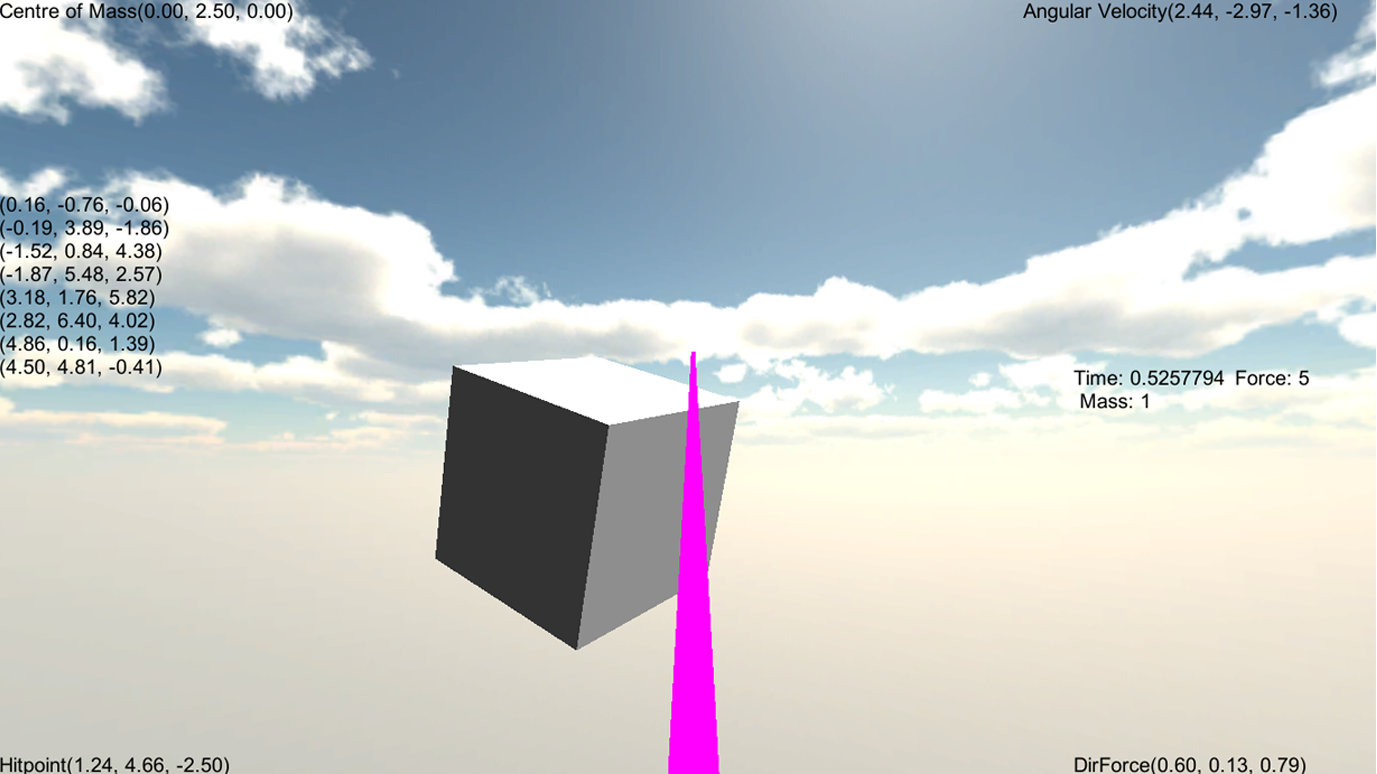
\includegraphics[width=\textwidth]{images/Screenshot2.PNG}
	\caption{Screenshot of Cube at $t = 0.526 s$}
	\label{fig:ScreenShotSingle}
\end{figure}
\begin{equation}\label{var:Rotation Variables}
	\boldsymbol{\omega} = 
	\begin{bmatrix}
		 2.44 \\
		-2.97 \\
		-1.36 
	\end{bmatrix}
	\qquad
	\mathbf{F} = f
	\begin{bmatrix}
		 0.6  \\
		 0.13 \\
		 0.79 
	\end{bmatrix}
	\qquad
	\tilde{\mathbf{p}_{0}} = 
	\begin{bmatrix}
		-2.5 \\
		 0 	 \\
		-2.5 
	\end{bmatrix}
\end{equation}
\begin{equation}\label{var:ftm}
	f = 5N
	\qquad
	t = 0.526s
	\qquad
	M = 1kg
\end{equation}
\begin{equation}\label{var:thetaomega}
	\omega = |\boldsymbol\omega| = 4.077
	\qquad
	\theta = \omega t = 2.144
\end{equation}
To start first acceleration will have to be calculated this will be represented by $\mathbf{A}$.
It will be calculated as mentioned before using Newton’s Second Law $F=MA$.
This means $\mathbf{A} = \mathbf{F}/M$ and results in Equation \ref{eq:Acceleration}.
\begin{equation}\label{eq:Acceleration}
	\mathbf{A} = \frac{f}{M}
	\begin{bmatrix}
		 0.6  \\
		 0.13 \\
		 0.79 
	\end{bmatrix} = 5
	\begin{bmatrix}
		 0.6  \\
		 0.13 \\
		 0.79 
	\end{bmatrix} = 
	\begin{bmatrix}
		 3  \\
		 0.65 \\
		 3.95 
	\end{bmatrix}
\end{equation}
The next step is to calculate the matrix $R$, which is a standard rotational matrix about any axis.
Equation \ref{ma:GeneralRotation} is the initial matrix that will be used. $C$ is shorthand for $(1-\cos\theta)$.
Below the rotational matrix are the values for $\alpha, \beta, \gamma$ in Equation \ref{var:alphabetagamma} and in Equation \ref{var:cs1-c} are the values of $\cos\theta, \sin\theta, (1-\cos\theta)$.
\begin{equation}\label{ma:GeneralRotation}
	R = 
	\begin{bmatrix}
		{\alpha}^{2}(C) + \cos\theta & 
		\alpha\beta(C) - \gamma\sin\theta & 
		\alpha\gamma(C) + \beta\sin\theta \\
		
		\alpha\beta(C) + \gamma\sin\theta & 
		{\beta}^{2}(C) + \cos\theta & 
		\beta\gamma(C) - \alpha\sin\theta \\
		
		\alpha\gamma(C) - \beta\sin\theta & 
		\beta\gamma(C) + \alpha\sin\theta & 
		{\gamma}^{2}(C) + \cos\theta \\
	\end{bmatrix}
\end{equation}
\begin{equation}\label{var:alphabetagamma}
	\alpha = \frac{\boldsymbol\omega_{x}}{\omega} = 0.5984
	\qquad
	\beta = \frac{\boldsymbol\omega_{y}}{\omega} = -0.7284
	\qquad
	\gamma = \frac{\boldsymbol\omega_{z}}{\omega} = -0.3336
\end{equation}
\begin{equation}\label{var:cs1-c}
	\cos\theta = -0.5421
	\qquad
	\sin\theta = 0.8403
	\qquad
	1-\cos\theta = 1.5421
\end{equation}
After substituting $\alpha, \beta, \gamma,\cos\theta, \sin\theta$, and $(1-\cos\theta)$ into the matrix the result can be seen in Matrix \ref{ma:Calculated Rotation}. Now multiply $R$ and $\tilde{\mathbf{p}_{0}}$ together to get Vector \ref{ma:CalculatedRPO}.
\begin{equation}\label{ma:Calculated Rotation}
	R = 
		\begin{bmatrix}
		   0.0102 & 
		  -0.392 & 
		  -0.9199 \\
		  
		  -0.9525 & 
		   0.2761 & 
		  -0.1282 \\
		  
		   0.3043 & 
		   0.8776 & 
		  -0.3705 \\
	\end{bmatrix}
\end{equation}
\begin{equation}\label{ma:CalculatedRPO}
	R\tilde{\mathbf{p}_{0}} = 
	\begin{bmatrix}
		 -2.2744 \\
		 -2.7018 \\
		 -0.1656 
	\end{bmatrix}
\end{equation}
$R\tilde{\mathbf{p}_{0}}$, $\mathbf{A}$, and $t^{2}$ can be substituted back into Equation \ref{eq:PositionGM} to find the final position of the chosen point.
\begin{equation}\label{eq:workout}
	\mathbf{p}=\frac{1}{2}
	\begin{bmatrix}
		 3  \\
		 0.65 \\
		 3.95 
	\end{bmatrix}
	0.526^{2}+
	\begin{bmatrix}
		 -2.2744 \\
 		 -2.7018 \\
 		 -0.1656 
	\end{bmatrix}
\end{equation}
\begin{equation}\label{eq:working2}
	\mathbf{p}=
	\begin{bmatrix}
		 0.4145  \\
		 0.0898  \\
		 0.5158 
	\end{bmatrix}
	+
	\begin{bmatrix}
		-2.2744 \\
 		-2.7018 \\
 		-0.1656 
	\end{bmatrix}
\end{equation}
\begin{equation}\label{eq:final}
	\mathbf{p}=
	\begin{bmatrix}
		-1.86  \\
		-2.61  \\
		 0.38 
	\end{bmatrix}
\end{equation}
\begin{figure}[h!]
	\centering
	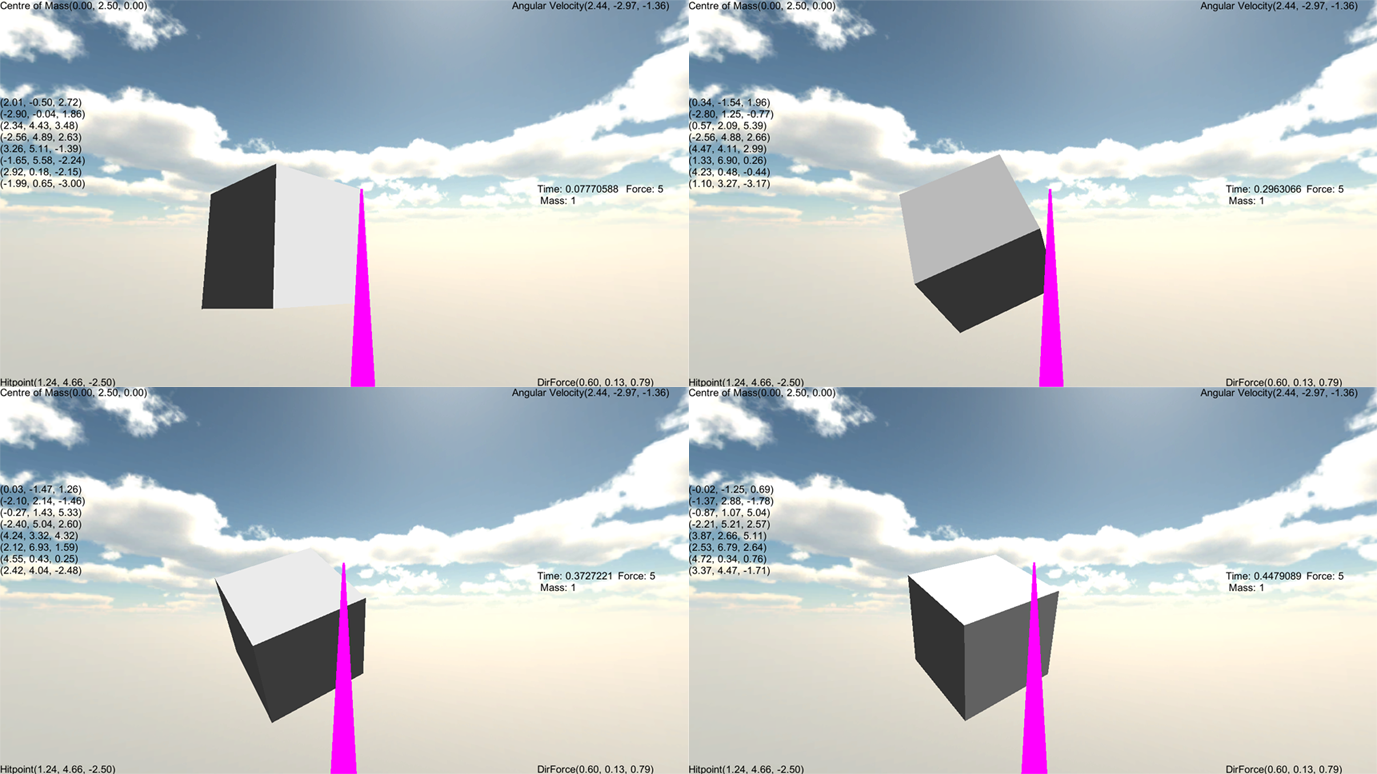
\includegraphics[width=\textwidth]{images/Screenshot1.PNG}
	\caption{Screenshot of Cube at $t = 0.078 s$, $t = 0.296 s$, $t = 0.373 s$, $t = 0.498 s$}
	\label{fig:ScreenShotFour}
\end{figure}
\begin{table}[ht]
	\caption{Position Comparison}		% title of Table
	\centering							% used for centering table
	\begin{tabular}{c c c c}			% centered columns (4 columns)
		\hline\hline 					%inserts double horizontal lines
		t (seconds) & Calculated Position & Application Position & Error Vector\\[0.5ex]% inserts table
		%heading
		\hline									% inserts single horizontal line
		0.078 & $(1.84,-0.75,2.94)$ & $(2.01,-0.5,2.72)$ & $(0.17,0.25,-0.22)$ \\
		0.296 & $(-0.43,-2.46,2.62)$ & $(0.34,-1.54,1.96)$ & $(0.77,0.92,-0.66)$ \\
		0.373 & $(-1.11,-2.74,2.01)$ & $(0.03,-1.47,1.26)$ & $(1.14,1.27,-0.75)$ \\
		0.448 & $(-1.6,-2.8,1.25)$ & $(-0.02,-1.25,0.69)$ & $(1.58,1.55,-0.56)$ \\
		0.526 & $(-1.86,-2.61,0.38)$ & $(0.16,-0.76,-0.06)$ & $(2.02,1.85,-0.44)$ \\ [1ex]	% [1ex] adds vertical space
		\hline									%inserts single line
	\end{tabular}
	\label{(table:ErrorTable)}					% is used to refer this table in the text
\end{table}